% =============================================================================
%  Integrated System Report
%  HyperLocal eCommerce Platform  +  VegPrice AI Prediction Engine
%  Complete Technical and Operational Documentation
%  Compile: pdflatex main.tex  (run twice for TOC and cross-references)
% =============================================================================

\documentclass[12pt, a4paper, oneside]{report}

% ─── Typography ───────────────────────────────────────────────────────────────
\usepackage[T1]{fontenc}
\usepackage[utf8]{inputenc}
\usepackage{palatino}
\usepackage{microtype}
\usepackage{setspace}
\onehalfspacing

% ─── Page Layout ──────────────────────────────────────────────────────────────
\usepackage[
  top    = 2.5cm,
  bottom = 2.5cm,
  left   = 3.2cm,
  right  = 2.5cm,
  headheight = 15pt,
]{geometry}

% ─── Chapter / Section Headings ───────────────────────────────────────────────
\usepackage{titlesec}

\titleformat{\chapter}[display]
  {\normalfont\Large\bfseries}
  {\rule[0.5ex]{\textwidth}{1.0pt}\\[4pt]%
   \normalsize\normalfont Chapter \thechapter}
  {4pt}{\huge\bfseries}
  [\vspace{6pt}\rule{\textwidth}{0.4pt}]
\titlespacing*{\chapter}{0pt}{-10pt}{24pt}

\titleformat{\section}
  {\normalfont\large\bfseries}{\thesection}{1em}{}
  [\vspace{-6pt}\rule{\textwidth}{0.3pt}]
\titlespacing*{\section}{0pt}{18pt}{6pt}

\titleformat{\subsection}
  {\normalfont\normalsize\bfseries}{\thesubsection}{1em}{}
\titlespacing*{\subsection}{0pt}{12pt}{4pt}

\titleformat{\subsubsection}
  {\normalfont\normalsize\itshape\bfseries}{\thesubsubsection}{1em}{}
\titlespacing*{\subsubsection}{0pt}{8pt}{2pt}

% ─── Headers and Footers ──────────────────────────────────────────────────────
\usepackage{fancyhdr}
\pagestyle{fancy}
\fancyhf{}
\fancyhead[L]{\small\nouppercase{\leftmark}}
\fancyhead[R]{\small\textit{HyperLocal + VegPrice AI --- Integrated Report}}
\fancyfoot[C]{\small\thepage}
\renewcommand{\headrulewidth}{0.4pt}
\fancypagestyle{plain}{\fancyhf{}\fancyfoot[C]{\small\thepage}\renewcommand{\headrulewidth}{0pt}}

% ─── Tables ───────────────────────────────────────────────────────────────────
\usepackage{booktabs}
\usepackage{tabularx}
\usepackage{longtable}
\usepackage{array}
\usepackage{multirow}
\renewcommand{\arraystretch}{1.30}

\newcolumntype{L}[1]{>{\raggedright\arraybackslash}p{#1}}
\newcolumntype{C}[1]{>{\centering\arraybackslash}p{#1}}
\newcolumntype{R}[1]{>{\raggedleft\arraybackslash}p{#1}}

% ─── Lists ────────────────────────────────────────────────────────────────────
\usepackage{enumitem}
\setlist[itemize]{leftmargin=2.2em, itemsep=2pt, topsep=4pt, parsep=0pt}
\setlist[enumerate]{leftmargin=2.2em, itemsep=2pt, topsep=4pt, parsep=0pt}
\setlist[description]{leftmargin=3.5cm, style=nextline, itemsep=4pt}

% ─── Code Listings ────────────────────────────────────────────────────────────
\usepackage{listings}
\lstdefinestyle{professional}{
  basicstyle       = \ttfamily\small,
  keywordstyle     = \bfseries,
  commentstyle     = \itshape,
  stringstyle      = \ttfamily,
  breaklines       = true,
  breakatwhitespace= true,
  frame            = single,
  framerule        = 0.5pt,
  xleftmargin      = 1.8em,
  xrightmargin     = 0.5em,
  aboveskip        = 0.8em,
  belowskip        = 0.8em,
  numbers          = left,
  numberstyle      = \tiny,
  numbersep        = 8pt,
  showstringspaces = false,
  tabsize          = 2,
  captionpos       = b,
}
\lstset{style=professional}

% ─── Framed Boxes ─────────────────────────────────────────────────────────────
\usepackage{mdframed}
\mdfdefinestyle{notebox}{
  linewidth        = 0.7pt,
  innerleftmargin  = 10pt, innerrightmargin = 10pt,
  innertopmargin   = 8pt,  innerbottommargin= 8pt,
  skipabove=6pt, skipbelow=6pt,
  frametitlefont   = \bfseries\small,
  frametitlerule   = true, frametitlerulewidth=0.4pt,
  frametitleaboveskip=3pt,
}
\newmdenv[style=notebox]{notebox}

% ─── Graphics and TikZ ────────────────────────────────────────────────────────
\usepackage{graphicx}
\usepackage{float}
\usepackage{tikz}
\usetikzlibrary{shapes.geometric,arrows.meta,positioning,fit,backgrounds,calc}

\tikzset{
  archnode/.style={rectangle,draw=black,thick,minimum width=2.4cm,
    minimum height=0.75cm,text centered,font=\small\bfseries,inner sep=4pt},
  shadednode/.style={archnode,fill=black!10},
  darknode/.style={archnode,fill=black!65,text=white},
  groupbox/.style={rectangle,draw=black,thick,rounded corners=4pt,inner sep=11pt},
  arrow/.style={-Stealth,thick},
  dblarrow/.style={Stealth-Stealth,thick},
  dasharrow/.style={-Stealth,thick,dashed},
}

% ─── Captions ─────────────────────────────────────────────────────────────────
\usepackage{caption}
\captionsetup{font=small,labelfont=bf,format=hang,margin=10pt}

% ─── TOC / Hyperref ───────────────────────────────────────────────────────────
\setcounter{tocdepth}{2}
\setcounter{secnumdepth}{3}
\usepackage[hidelinks,
  pdftitle ={HyperLocal eCommerce + VegPrice AI --- Integrated Report},
  pdfauthor={Nitheesh D R},
]{hyperref}

\usepackage{amsmath}
\usepackage{parskip}

% =============================================================================
\begin{document}
% =============================================================================

% ─── Title Page ───────────────────────────────────────────────────────────────
\begin{titlepage}
\centering
\vspace*{1.6cm}

{\large\scshape Complete Technical \& Operational Documentation}

\vspace{0.6cm}
\rule{\textwidth}{1.4pt}\\[0.5cm]

{\fontsize{30}{38}\selectfont\bfseries HyperLocal eCommerce Platform}

\vspace{0.3cm}
{\Large \&}

\vspace{0.3cm}
{\fontsize{26}{34}\selectfont\bfseries VegPrice AI Prediction Engine}

\vspace{0.4cm}
{\large Integrated Intelligent Ordering and Delivery System}

\vspace{0.4cm}
\rule{\textwidth}{0.6pt}

\vspace{1.8cm}

\begin{tabular}{@{} R{4.4cm} @{\quad} L{8.8cm} @{}}
\textbf{System Type}     & Multi-Vendor Hyperlocal eCommerce + AI Price Prediction \\[6pt]
\textbf{Customer App}    & React Native (iOS \& Android) + Progressive Web App \\[6pt]
\textbf{Seller App}      & React Native Mobile App + Web Panel (Admin/Seller) \\[6pt]
\textbf{Delivery App}    & React Native Rider Application \\[6pt]
\textbf{Prediction API}  & Vercel Serverless (Python) + NVIDIA NIM LLM \\[6pt]
\textbf{Database}        & Supabase (PostgreSQL) + eCommerce DB \\[6pt]
\textbf{Author}          & Nitheesh D R \\[6pt]
\textbf{Date}            & April 2026 \\
\end{tabular}

\vfill

\begin{tabular}{@{} C{2.4cm} C{0.3cm} C{2.4cm} C{0.3cm} C{2.4cm} C{0.3cm} C{2.4cm} @{}}
React Native & $\cdot$ & FastAPI & $\cdot$ & Supabase & $\cdot$ & NVIDIA NIM \\[4pt]
XGBoost      & $\cdot$ & LightGBM & $\cdot$ & Prophet & $\cdot$ & Vercel \\[4pt]
Firebase FCM & $\cdot$ & Redis   & $\cdot$ & Docker  & $\cdot$ & EAS Build \\
\end{tabular}

\vspace{1.2cm}
\rule{\textwidth}{0.4pt}\\[0.3cm]
{\small\itshape
  This report documents the end-to-end architecture, working process, and technical\\
  implementation of the integrated HyperLocal eCommerce and price prediction system.
}\\[0.3cm]
\rule{\textwidth}{1.0pt}
\end{titlepage}

% ─── Abstract ─────────────────────────────────────────────────────────────────
\chapter*{Abstract}
\addcontentsline{toc}{chapter}{Abstract}

This report documents the complete architecture and operational workflow of an
integrated system comprising two major components: the \textbf{HyperLocal
eCommerce Platform} and the \textbf{VegPrice AI Prediction Engine}.

The HyperLocal platform is a multi-vendor hyperlocal commerce system supporting
independent sellers, geofenced delivery zones, a customer-facing mobile app and
web portal, a seller management app and panel, a rider delivery app, and a
centralised admin panel. It enables vendors to list vegetables and perishable
goods for local delivery within defined zone boundaries.

The VegPrice AI Prediction Engine is a machine-learning and large language model
pipeline that collects historical price data from the eCommerce platform, trains
an ensemble of five regression models (XGBoost, LightGBM, Prophet, LSTM, and
Linear Regression), and generates next-day price forecasts augmented by NVIDIA
NIM LLM contextual reasoning. These predictions are written back to the
eCommerce database, surfaced in the customer-facing interfaces, and used by the
system to suggest optimal ordering times.

The integration creates a closed feedback loop: the eCommerce platform is the
source of truth for price records; the AI engine consumes that data, produces
forecasts, and publishes them back; customers see price forecasts before ordering
and receive smart buy-now or wait recommendations; orders are placed and
dispatched through the hyperlocal delivery network.

\noindent\textbf{Keywords:} hyperlocal eCommerce, multi-vendor marketplace,
vegetable price prediction, machine learning ensemble, NVIDIA NIM, React Native,
FastAPI, Supabase, geofencing, delivery zones, order management.

% ─── Front Matter ─────────────────────────────────────────────────────────────
\tableofcontents
\newpage
\listoftables
\addcontentsline{toc}{chapter}{List of Tables}
\newpage

% =============================================================================
\chapter{Executive Summary}
% =============================================================================

\section{Project Overview}

This project combines a production-grade hyperlocal eCommerce platform with an
intelligent price prediction engine to create a data-driven marketplace for
fresh vegetables and perishable goods. The system operates as a closed loop:

\begin{enumerate}
  \item The \textbf{HyperLocal eCommerce Platform} enables sellers to list
        vegetables, manage inventory, and fulfil orders within geofenced delivery
        zones. Every transaction generates price records stored in the platform
        database.
  \item The \textbf{VegPrice AI Prediction Engine} periodically extracts price
        records from the eCommerce database, retrains ML models, and generates
        next-day price forecasts using an ensemble of five regression models
        augmented by NVIDIA NIM LLM contextual reasoning.
  \item Forecasts are published back to the eCommerce platform through a REST
        API. The customer-facing interfaces display price predictions alongside
        product listings, enabling users to see whether a price is likely to
        rise or fall before placing an order.
  \item When a customer places an order, the hyperlocal delivery network
        dispatches a rider within the geofenced zone. The Rider App provides
        live route tracking, one-tap order acceptance, and earnings management.
\end{enumerate}

\section{Business Value}

\begin{table}[H]
\centering
\caption{Business Value by Stakeholder}
\label{tab:business-value}
\begin{tabularx}{\textwidth}{@{} L{2.8cm} X @{}}
\toprule
\textbf{Stakeholder} & \textbf{Value Delivered} \\
\midrule
Customers
  & See tomorrow's predicted price before ordering; receive a buy-now or
    wait recommendation; track delivery live on a geofenced map. \\[4pt]
Sellers
  & Subscription-based storefront; multi-store management; role-based
    staff access; AI price signals guide restocking decisions. \\[4pt]
Delivery Riders
  & One-tap order acceptance; live route optimisation within delivery zones;
    real-time earnings tracking and wallet withdrawals. \\[4pt]
Administrators
  & Full oversight of sellers, products, orders, delivery zones, commissions,
    promotions, tax rules, and push notifications from a single panel. \\[4pt]
Platform Owner
  & Commission revenue per order; seller subscription revenue; data asset
    (historical price records) that continuously improves prediction accuracy. \\
\bottomrule
\end{tabularx}
\end{table}

\section{System Component Summary}

\begin{table}[H]
\centering
\caption{System Component Overview}
\label{tab:components}
\begin{tabularx}{\textwidth}{@{} L{3.5cm} X @{}}
\toprule
\textbf{Component} & \textbf{Description} \\
\midrule
Customer Mobile App    & React Native iOS/Android app; browse, order, track delivery. \\
Customer Web           & Progressive web app; full eCommerce experience in browser. \\
Seller Mobile App      & React Native app; manage products, orders, earnings, inventory. \\
Seller Web Panel       & Browser-based panel; full store, product, and settlement management. \\
Rider/Delivery App     & React Native app; accept orders, navigate routes, manage earnings. \\
Admin Panel            & Web panel; manage all sellers, zones, tax, promos, notifications. \\
VegPrice AI API        & Vercel serverless Python API; predictions via ML ensemble + NIM. \\
Supabase Database      & Prediction storage; price records; alert subscriptions. \\
eCommerce Database     & Order records; inventory; user data; seller data. \\
\bottomrule
\end{tabularx}
\end{table}

% =============================================================================
\chapter{Integrated System Architecture}
% =============================================================================

\section{High-Level Architecture}

The two systems communicate through a bidirectional REST API bridge. The
eCommerce platform is the primary data source and consumer; the AI engine is
the prediction processor.

\begin{figure}[H]
\centering
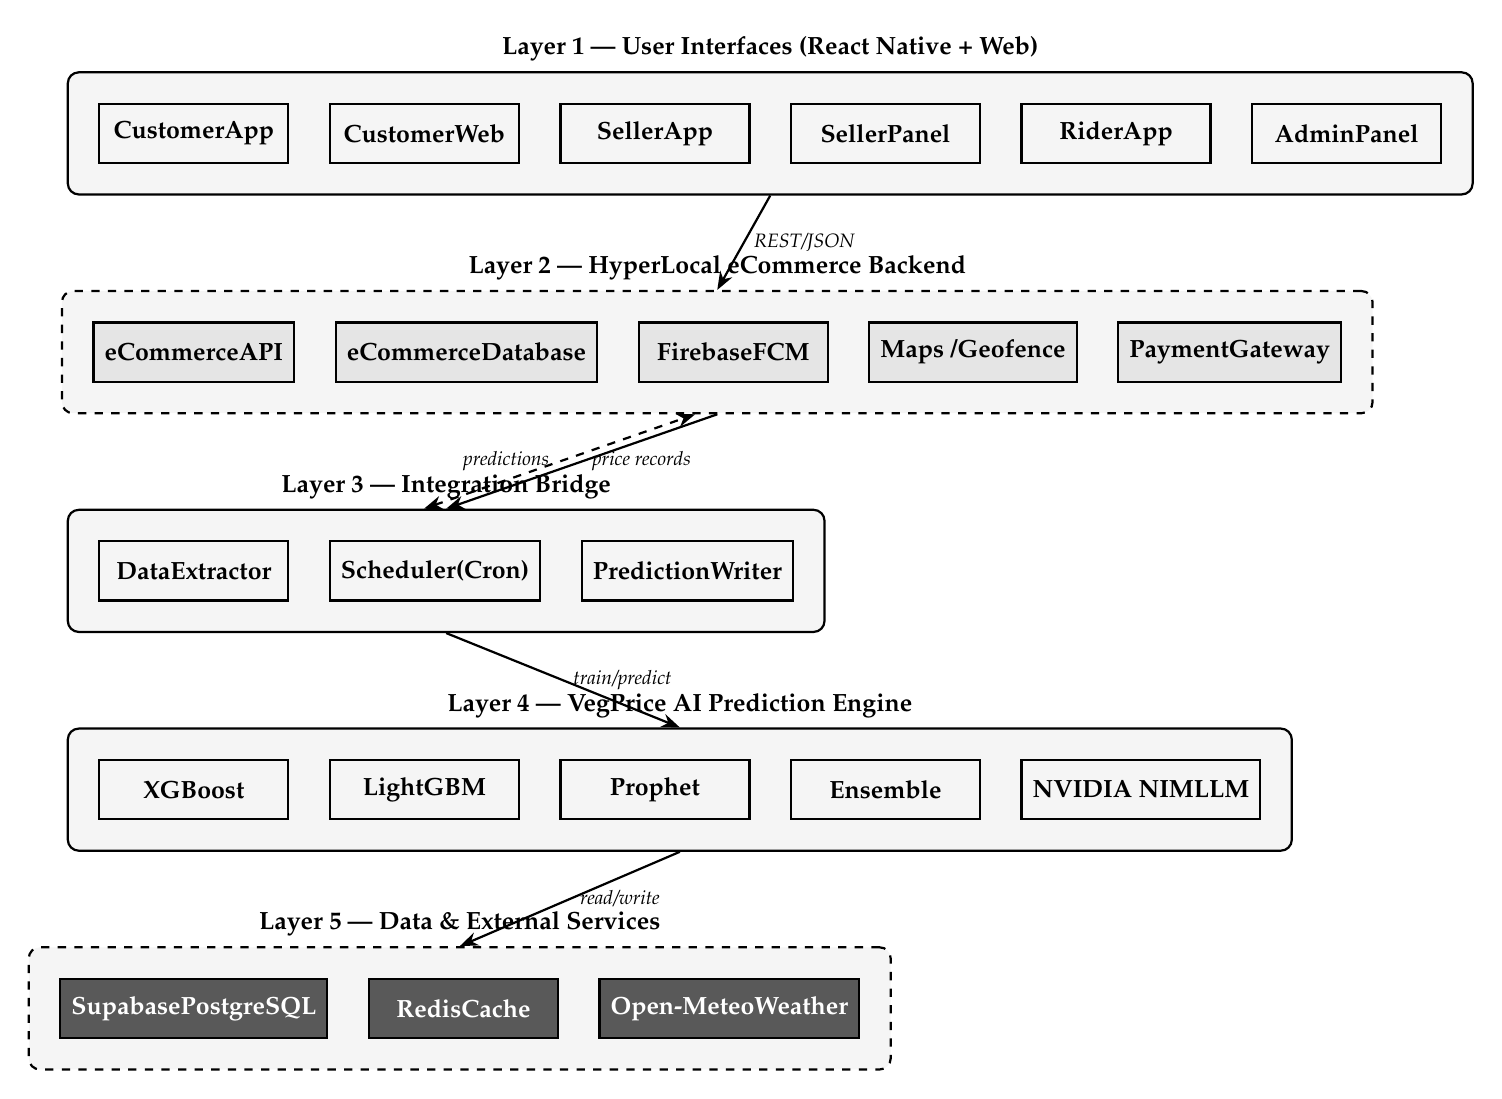
\begin{tikzpicture}[node distance=1.8cm and 0.5cm]

  %% ── Layer 1: Customer Interfaces ──────────────────────────────────────────
  \node[archnode] (custapp)  {Customer\\App};
  \node[archnode, right=0.5cm of custapp]  (custweb)  {Customer\\Web};
  \node[archnode, right=0.5cm of custweb]  (selapp)   {Seller\\App};
  \node[archnode, right=0.5cm of selapp]   (selpanel) {Seller\\Panel};
  \node[archnode, right=0.5cm of selpanel] (riderapp) {Rider\\App};
  \node[archnode, right=0.5cm of riderapp] (admin)    {Admin\\Panel};
  \begin{scope}[on background layer]
    \node[groupbox,fill=black!4,
      fit=(custapp)(admin),
      label={[font=\small\bfseries]above:Layer 1 \textemdash{} User Interfaces (React Native + Web)}]
      (ui) {};
  \end{scope}

  %% ── Layer 2: eCommerce Backend ────────────────────────────────────────────
  \node[shadednode, below=2cm of custapp]  (ecapi)  {eCommerce\\API};
  \node[shadednode, right=0.5cm of ecapi]  (ecdb)   {eCommerce\\Database};
  \node[shadednode, right=0.5cm of ecdb]   (fcm)    {Firebase\\FCM};
  \node[shadednode, right=0.5cm of fcm]    (maps)   {Maps /\\Geofence};
  \node[shadednode, right=0.5cm of maps]   (pay)    {Payment\\Gateway};
  \begin{scope}[on background layer]
    \node[groupbox,fill=black!4,dashed,
      fit=(ecapi)(pay),
      label={[font=\small\bfseries]above:Layer 2 \textemdash{} HyperLocal eCommerce Backend}]
      (ec) {};
  \end{scope}

  %% ── Layer 3: AI Bridge ────────────────────────────────────────────────────
  \node[archnode, below=2cm of ecapi]  (bridge) {Data\\Extractor};
  \node[archnode, right=0.5cm of bridge](sched)  {Scheduler\\(Cron)};
  \node[archnode, right=0.5cm of sched] (writer) {Prediction\\Writer};
  \begin{scope}[on background layer]
    \node[groupbox,fill=black!4,
      fit=(bridge)(writer),
      label={[font=\small\bfseries]above:Layer 3 \textemdash{} Integration Bridge}]
      (intg) {};
  \end{scope}

  %% ── Layer 4: AI Engine ────────────────────────────────────────────────────
  \node[archnode, below=2cm of bridge] (xgb)    {XGBoost};
  \node[archnode, right=0.5cm of xgb]  (lgbm)   {LightGBM};
  \node[archnode, right=0.5cm of lgbm] (prophet){Prophet};
  \node[archnode, right=0.5cm of prophet](ens)  {Ensemble};
  \node[archnode, right=0.5cm of ens]  (nim)    {NVIDIA NIM\\LLM};
  \begin{scope}[on background layer]
    \node[groupbox,fill=black!4,
      fit=(xgb)(nim),
      label={[font=\small\bfseries]above:Layer 4 \textemdash{} VegPrice AI Prediction Engine}]
      (ai) {};
  \end{scope}

  %% ── Layer 5: Data Stores ──────────────────────────────────────────────────
  \node[darknode, below=2cm of xgb]    (pg)     {Supabase\\PostgreSQL};
  \node[darknode, right=0.5cm of pg]   (redis)  {Redis\\Cache};
  \node[darknode, right=0.5cm of redis](weather){Open-Meteo\\Weather};
  \begin{scope}[on background layer]
    \node[groupbox,fill=black!4,dashed,
      fit=(pg)(weather),
      label={[font=\small\bfseries]above:Layer 5 \textemdash{} Data \& External Services}]
      (data) {};
  \end{scope}

  %% ── Arrows ────────────────────────────────────────────────────────────────
  \draw[arrow] (ui.south)   -- node[right,font=\scriptsize\itshape]{REST/JSON}     (ec.north);
  \draw[arrow] (ec.south)   -- node[right,font=\scriptsize\itshape]{price records} (intg.north);
  \draw[arrow] (intg.south) -- node[right,font=\scriptsize\itshape]{train/predict} (ai.north);
  \draw[arrow] (ai.south)   -- node[right,font=\scriptsize\itshape]{read/write}    (data.north);

  %% ── Feedback arrow: predictions back to eCommerce ─────────────────────────
  \draw[dblarrow,dashed] ([xshift=-8pt]intg.north) -- ([xshift=-8pt]ec.south)
    node[midway,left,font=\scriptsize\itshape]{predictions};

\end{tikzpicture}
\caption{Five-layer integrated system architecture}
\label{fig:architecture}
\end{figure}

\section{Integration Data Flow Overview}

\begin{table}[H]
\centering
\caption{Cross-System Data Flow}
\label{tab:data-flow}
\begin{tabularx}{\textwidth}{@{} C{0.6cm} L{3.8cm} X @{}}
\toprule
\textbf{Step} & \textbf{Action} & \textbf{Detail} \\
\midrule
1 & Sellers list products
  & Sellers add vegetables with prices via the Seller App or Panel. The
    eCommerce API writes product and price records to the eCommerce
    database. \\[3pt]
2 & Customers place orders
  & Customers browse, see AI price forecasts, and place orders. Order
    records and transaction prices are logged in the eCommerce database. \\[3pt]
3 & Data extraction (nightly)
  & The Integration Bridge cron job queries the eCommerce database for
    new \texttt{price\_records} since the last run and writes them to
    Supabase \texttt{price\_records}. \\[3pt]
4 & ML model retraining
  & The VegPrice AI scheduler triggers retraining of all five model
    classes for each vegetable using the updated Supabase dataset. \\[3pt]
5 & Prediction generation
  & The ensemble model and NVIDIA NIM LLM generate next-day price
    forecasts with confidence intervals. Predictions are saved to Supabase
    \texttt{predictions}. \\[3pt]
6 & Prediction publish
  & The Prediction Writer calls the eCommerce API's price-forecast endpoint
    (\texttt{POST /api/product/price-forecast}) with the AI predictions.
    The eCommerce database stores these as forecast records. \\[3pt]
7 & Customer visibility
  & The Customer App and Web display the forecast alongside the current
    product price. A buy-now or wait recommendation badge is shown. \\[3pt]
8 & Order and delivery
  & Customer places order; rider accepts and navigates to seller, then
    customer. Delivery is tracked live on the geofenced map. \\
\bottomrule
\end{tabularx}
\end{table}

% =============================================================================
\chapter{HyperLocal eCommerce Platform}
% =============================================================================

\section{Platform Overview}

The HyperLocal eCommerce Platform is a multi-vendor marketplace designed for
local, zone-based commerce. It supports two operating modes:

\begin{description}
  \item[Multi-Vendor Mode]
    Multiple independent sellers each manage their own stores. The platform
    owner earns a configurable commission per order. Customers can order from
    multiple stores in a single checkout.
  \item[Single Vendor Mode]
    The platform is configured as a single-store eCommerce system with one
    owner. This mode is selected once at setup and cannot be changed later.
\end{description}

\section{Platform Components}

\begin{table}[H]
\centering
\caption{Platform Components and Target Users}
\label{tab:platform-components}
\begin{tabularx}{\textwidth}{@{} L{3.2cm} L{2.5cm} X @{}}
\toprule
\textbf{Component} & \textbf{Stack} & \textbf{Target User and Purpose} \\
\midrule
Customer Mobile App & React Native & End-consumers; browse categories, place orders,
  track delivery, manage wishlist and addresses. \\[4pt]
Customer Web Portal & React / PWA  & End-consumers on desktop/browser; full shopping
  experience including geolocation, filters, cart, checkout. \\[4pt]
Seller Mobile App   & React Native & Sellers and staff on mobile; manage products,
  orders, inventory, earnings, FAQs, and notifications. \\[4pt]
Seller Web Panel    & React / Web  & Sellers on desktop; complete store management,
  product attributes, categories, wallet, settlements, and returns. \\[4pt]
Rider/Delivery App  & React Native & Delivery personnel; accept orders, navigate
  routes, manage earnings wallet and withdrawal history. \\[4pt]
Admin Panel         & React / Web  & Platform administrators; manage all sellers,
  zones, tax rules, banners, promos, roles, and notifications. \\
\bottomrule
\end{tabularx}
\end{table}

\section{Admin Panel}

The Admin Panel provides centralised control over the entire platform.

\subsection{Dashboard}

Displays real-time KPIs: total orders, total revenue, active sellers, registered
customers, pending product approvals, active riders, and commission earned for
the current period. Charts visualise daily order volume and revenue trends.

\subsection{Seller Management}

Administrators can view, approve, suspend, or permanently ban seller accounts.
Each seller profile shows subscription plan, associated stores, outstanding
commissions, and a log of recent activity.

\subsection{Subscription Plans}

The platform supports tiered seller subscription plans (e.g., Free, Basic,
Pro). The admin panel allows creation and management of plans with features
such as maximum product listings, store count, analytics access, and badge
visibility.

\subsection{Single Vendor / Multi Vendor Toggle}

A one-time configuration flag switches the platform between single-vendor and
multi-vendor mode. This setting is irreversible once set and controls whether
commission logic, multi-store checkout, and seller-facing features are active.

\subsection{Category Management}

Admins create and organise the top-level product category tree. Categories
include custom icons, banners, and ordering weight. Sellers assign their products
to one or more admin-defined categories.

\subsection{Delivery Zone Management}

Geofenced delivery zones are drawn on a map interface. Each zone has:
\begin{itemize}
  \item Name, colour, and activation status.
  \item A polygon boundary defined by GPS coordinates.
  \item Per-zone delivery fee rules and minimum order values.
  \item A list of assigned stores whose inventory is available within that zone.
\end{itemize}

\subsection{Order Commission}

Commission rates are configured per category or globally. Charts show commission
earned per seller and per category over selectable date ranges. Settlement
requests from sellers are reviewed and approved in this section.

\subsection{Tax Rate Management}

A tax and fee rule engine allows the admin to define:
\begin{itemize}
  \item Percentage or flat-fee tax rates per product category.
  \item Inclusive or exclusive tax application.
  \item Zone-specific tax overrides.
\end{itemize}

\subsection{Product Approval}

All new product listings submitted by sellers require admin approval before
becoming visible to customers. The admin can approve, reject, or request
changes with a reason note.

\subsection{Promotions and Banners}

\begin{itemize}
  \item \textbf{Banners}: Upload and schedule promotional banners for the
        customer app and web home page.
  \item \textbf{Promos}: Create discount codes with percentage or flat value,
        minimum order value, usage limits, and expiry dates.
  \item \textbf{Featured Section}: Dynamically configure which products or
        categories appear in the featured section on the customer home screen.
\end{itemize}

\subsection{Notification Management}

Send push notifications to all customers, all sellers, all riders, or targeted
segments. Custom SMS integration is supported for OTP and order-status messages.

\subsection{Roles and Permissions}

Sub-administrator accounts are created with granular permission sets. Each
permission toggles access to a specific admin panel section (e.g., read-only
orders, manage sellers, manage zones).

\section{Seller App and Panel}

\subsection{Seller Mobile App}

The Seller Mobile App is a React Native application for on-the-go store
management.

\begin{table}[H]
\centering
\caption{Seller Mobile App Screens}
\label{tab:seller-app-screens}
\begin{tabularx}{\textwidth}{@{} L{3.6cm} X @{}}
\toprule
\textbf{Screen} & \textbf{Functionality} \\
\midrule
Smart Dashboard
  & KPI summary: today's orders, pending orders, total earnings, low-stock
    alerts, and recent activity feed. \\[4pt]
Product Management
  & Add, edit, or deactivate product listings. Set price, variants (size,
    weight), images, FAQs, and stock quantity. \\[4pt]
Store Management
  & Configure store name, logo, address, operating hours, delivery zones
    served, and store verification status. \\[4pt]
Order Management
  & View incoming orders, update order status (confirmed, preparing, ready,
    dispatched), and communicate with customers. \\[4pt]
Earnings Overview
  & Daily/weekly/monthly earnings charts; settlement history; outstanding
    balance pending withdrawal. \\[4pt]
Brands Management
  & Create and manage product brands associated with the store. \\[4pt]
Categories Management
  & Assign products to admin-defined categories; create sub-categories. \\[4pt]
Tax Rates
  & View and set product-level tax rate overrides where permitted. \\[4pt]
Roles \& Permissions
  & Create staff accounts with limited access scopes (e.g., order-only view). \\[4pt]
Subscription Plans
  & View current plan, upgrade options, and plan expiry. \\[4pt]
Smart Notification
  & Receive real-time push notifications for new orders, low stock, and
    settlement updates. \\
\bottomrule
\end{tabularx}
\end{table}

\subsection{Seller Web Panel}

The Seller Web Panel is a browser-based management interface providing full
desktop access to all seller functions.

\begin{table}[H]
\centering
\caption{Seller Web Panel Sections}
\label{tab:seller-panel}
\begin{tabularx}{\textwidth}{@{} L{3.6cm} X @{}}
\toprule
\textbf{Section} & \textbf{Functionality} \\
\midrule
Seller Dashboard    & Full KPI dashboard with charts; order trends; revenue analytics. \\[4pt]
Subscription Plan   & View active plan; upgrade or renew via integrated payment. \\[4pt]
Stores Management   & Multi-store creation and configuration; operating hours; zone assignment. \\[4pt]
Manage Products     & Bulk product management; CSV import/export; variant matrix. \\[4pt]
Product Attributes  & Define custom attribute sets (e.g., weight options, freshness grade). \\[4pt]
Categories          & Hierarchical category management for the seller's product catalogue. \\[4pt]
Order Management    & Full order lifecycle view; status updates; customer communication. \\[4pt]
Wallet \& Settlements & Real-time wallet balance; request settlement; view payout history. \\[4pt]
Settlement History  & Detailed log of all approved and pending settlement requests. \\[4pt]
Brands Management   & Brand creation with logo and description. \\[4pt]
Return Management   & Handle product return requests; approve or reject returns. \\[4pt]
Tax Rates           & Configure tax rates for specific products or categories. \\[4pt]
Roles \& Permissions& Create and manage staff user accounts with permission scopes. \\[4pt]
Seller Notifications& View and configure which notification types trigger push/SMS alerts. \\
\bottomrule
\end{tabularx}
\end{table}

\section{Customer App and Web}

\subsection{Customer Mobile App}

The Customer Mobile App is a React Native application covering the complete
shopping journey from discovery to delivery.

\begin{table}[H]
\centering
\caption{Customer App Key Screens and Features}
\label{tab:customer-app}
\begin{tabularx}{\textwidth}{@{} L{3.6cm} X @{}}
\toprule
\textbf{Screen / Feature} & \textbf{Description} \\
\midrule
Home / Categories
  & Curated category grid, dynamic featured sections, promotional banners,
    top-selling products, and AI price-trend badges. \\[4pt]
Nearby Stores View
  & Map-based store discovery using device location and geofenced zone detection. \\[4pt]
Product Listing
  & Filterable and searchable product list with smart search suggestions,
    brand filter, category filter, and price-range slider. \\[4pt]
Product Detail
  & Full product information, variant selector, FAQ accordion, seller info,
    ratings and reviews, and delivery availability within zone. \\[4pt]
\textbf{AI Price Forecast}
  & Tomorrow's predicted price shown below current price; buy-now or wait
    recommendation badge; 7-day trend chart powered by VegPrice AI. \\[4pt]
Add to Cart / Buy Now
  & Quick add to cart or one-click Buy Now checkout flow. \\[4pt]
Shopping List Builder
  & Create and manage a planned purchase list separate from the live cart. \\[4pt]
Wishlist
  & Save products for later; notified when a wishlisted product price drops. \\[4pt]
Multi-Store Checkout
  & Seamless single checkout spanning products from multiple sellers. \\[4pt]
Promo Codes
  & Apply discount codes at checkout; real-time validation. \\[4pt]
Multiple Payment Options
  & Card, UPI, wallet, cash on delivery; configurable per zone. \\[4pt]
Live Order Tracking
  & Real-time map showing rider location within the geofenced delivery zone. \\[4pt]
Order Status \& History
  & Full order history with status timeline and receipt download. \\[4pt]
Ratings \& Reviews
  & Submit product and delivery reviews post-order. \\[4pt]
Multiple Addresses
  & Save and manage multiple delivery addresses with location pin. \\
\bottomrule
\end{tabularx}
\end{table}

\subsection{Customer Web Portal}

The Customer Web Portal is a progressive web application providing the
complete shopping experience in a browser. It mirrors the mobile app's feature
set with additional desktop-optimised layouts including:

\begin{itemize}
  \item \textbf{Intelligent search} with live product and category suggestions.
  \item \textbf{Automatic location detection} via browser Geolocation API.
  \item \textbf{Dynamic featured section builder} rendering admin-configured
        promotional blocks.
  \item \textbf{Shop by brands} horizontal scroll row.
  \item \textbf{Product variant selector} with stock availability indicators.
  \item \textbf{Delivery instructions and attachments} on the checkout page.
  \item \textbf{Available delivery zones display} showing which zones are
        currently active.
  \item \textbf{Custom product section} for platform-wide featured products.
\end{itemize}

\section{Rider / Delivery App}

The Rider App is a React Native application used by delivery personnel.

\begin{table}[H]
\centering
\caption{Rider App Features}
\label{tab:rider-app}
\begin{tabularx}{\textwidth}{@{} L{3.6cm} X @{}}
\toprule
\textbf{Feature} & \textbf{Description} \\
\midrule
Smart Dashboard
  & Overview of today's deliveries, active orders, completed orders, and
    earnings for the current session. \\[4pt]
Earnings Insights
  & Daily and weekly earnings charts; peak-hour analysis. \\[4pt]
My Orders
  & List of all pending and in-progress orders assigned to the rider. \\[4pt]
Order Details
  & Full order card: customer address, items, seller location, and customer
    contact. \\[4pt]
One-Tap Order Accept
  & Accept or reject incoming order assignments in real time. \\[4pt]
Live Delivery Route Tracking
  & Turn-by-turn map navigation constrained within the rider's assigned
    delivery zone using geofencing. \\[4pt]
Dark Mode
  & Full dark-mode UI for night-time deliveries. \\[4pt]
Earnings Wallet
  & Real-time wallet balance showing completed delivery payments. \\[4pt]
Withdrawal History
  & Log of all wallet withdrawal requests and their approval status. \\[4pt]
Smart Notifications
  & Push alerts for new order assignments, cancellations, and payment
    confirmations. \\
\bottomrule
\end{tabularx}
\end{table}

\section{Key Platform Features}

\begin{table}[H]
\centering
\caption{Complete Platform Feature Matrix}
\label{tab:features-matrix}
\begin{tabularx}{\textwidth}{@{} L{4.5cm} X @{}}
\toprule
\textbf{Feature} & \textbf{Description} \\
\midrule
Multi-Delivery Zones
  & Manage multiple geofenced service areas; per-zone delivery charges
    and minimum order values; zone-based store assignment. \\[3pt]
Seller Multi-Store Support
  & Each seller account can manage multiple physical store locations
    from a single login. \\[3pt]
Roles \& Permissions
  & Granular permission system for admin sub-accounts and seller staff
    accounts; access scoped to specific modules. \\[3pt]
Multi Tax System
  & Flexible tax rule engine; supports multiple rate types, inclusive/
    exclusive application, and category-level overrides. \\[3pt]
Seller Subscription
  & Admin-defined tiered subscription plans gate seller features; recurring
    revenue stream for the platform. \\[3pt]
Chat System
  & Real-time messaging between customers, sellers, and delivery partners
    using WebSocket. \\[3pt]
Commission Engine
  & Per-category or global commission rates; automatic deduction from
    seller earnings on order completion. \\[3pt]
Geofencing Delivery Map
  & GPS-polygon zone boundaries; riders and customers see zone boundaries
    on the map; out-of-zone orders blocked. \\[3pt]
Location-Based Store System
  & Only stores within the customer's detected zone are shown, reducing
    irrelevant listings. \\[3pt]
Live Order Tracking
  & Supabase Realtime pushes rider location updates to the customer app
    every 5 seconds during active delivery. \\[3pt]
Rider Self-Order Acceptance
  & Riders accept or reject assignments with a single tap; rejected orders
    are re-assigned to the next nearest available rider. \\[3pt]
Low Stock Alerts
  & Sellers and admins receive push notifications when product stock falls
    below a configurable threshold. \\[3pt]
Smart Preference Wishlist
  & Wishlist items trigger price-drop notifications and AI forecast alerts. \\[3pt]
Share Product \& Deep Linking
  & Shareable product URLs that open directly in the app or web with
    full product context. \\[3pt]
Custom SMS Integration
  & OTP, order confirmation, and status updates via configurable SMS
    gateway. \\[3pt]
Advanced Product Filtering
  & Faceted search across price range, brand, category, rating, and
    delivery availability. \\
\bottomrule
\end{tabularx}
\end{table}

% =============================================================================
\chapter{VegPrice AI Prediction Engine}
% =============================================================================

\section{Engine Overview}

The VegPrice AI Prediction Engine is a Python-based ML pipeline deployed on
Vercel Serverless for production and FastAPI for local development. It
consumes price data from the eCommerce platform, trains a five-model ensemble
per vegetable, and publishes predictions back to the eCommerce system and a
Supabase prediction store.

\section{Data Sources}

\begin{table}[H]
\centering
\caption{Prediction Engine Data Sources}
\label{tab:data-sources}
\begin{tabularx}{\textwidth}{@{} L{3.8cm} L{3.0cm} X @{}}
\toprule
\textbf{Source} & \textbf{Data Type} & \textbf{How Used} \\
\midrule
eCommerce Platform DB
  & Transaction price records & Primary training signal; seller-listed
    and transaction-settled prices per vegetable per date. \\[4pt]
Agmarknet / Kaggle Dataset
  & Historical mandi prices   & Initial model bootstrap; 3+ years of
    Chennai wholesale market data. \\[4pt]
Open-Meteo API
  & Real-time weather          & Contextual feature for LLM prompt and
    ML feature engineering (rainfall, temperature, humidity). \\[4pt]
Tamil Nadu Festival Calendar
  & Festival dates             & Binary ``is\_festival'' feature; festival
    days correlate with demand spikes and supply disruptions. \\[4pt]
Supabase \texttt{price\_records}
  & Unified price ledger       & Single source of truth after extraction
    from both eCommerce DB and Agmarknet. \\
\bottomrule
\end{tabularx}
\end{table}

\section{Feature Engineering}

\begin{table}[H]
\centering
\caption{Feature Engineering Specification}
\label{tab:features-eng}
\begin{tabularx}{\textwidth}{@{} L{3.0cm} L{4.8cm} X @{}}
\toprule
\textbf{Group} & \textbf{Features} & \textbf{Description} \\
\midrule
Lag features
  & \texttt{price\_lag\_1}, \texttt{price\_lag\_2},
    \texttt{price\_lag\_7}, \texttt{price\_lag\_14}
  & Modal prices from 1, 2, 7, and 14 days prior; captures short-term
    momentum. \\[4pt]
Rolling statistics
  & \texttt{rolling\_mean\_3}, \texttt{rolling\_mean\_7},
    \texttt{rolling\_mean\_14}, \texttt{rolling\_std\_7}
  & Moving averages and variance; encodes trend and volatility. \\[4pt]
Seasonal encoding
  & \texttt{doy\_sin}, \texttt{doy\_cos}
  & Sine/cosine of day-of-year; continuous cyclic annual seasonality. \\[4pt]
Calendar
  & \texttt{day\_of\_week}, \texttt{month},
    \texttt{is\_weekend}, \texttt{is\_festival}
  & Weekly market patterns and festival price effects. \\[4pt]
Weather
  & \texttt{temperature}, \texttt{rainfall\_mm},
    \texttt{humidity\_pct}
  & Weather from Open-Meteo merged by date. \\[4pt]
Supply proxy
  & \texttt{arrival\_qty},
    \texttt{supply\_demand\_ratio}
  & Arrival quantity vs.\ rolling average; supply shock signal. \\[4pt]
Market encoding
  & One-hot market columns
  & Per-market price differentials across Chennai mandis. \\
\bottomrule
\end{tabularx}
\end{table}

\section{Model Portfolio}

Five model classes are trained for each of the 18 supported vegetables
(18 $\times$ 5 = \textbf{90 model artefact files}).

\begin{table}[H]
\centering
\caption{ML Model Portfolio}
\label{tab:models}
\begin{tabularx}{\textwidth}{@{} L{3.0cm} L{3.0cm} X @{}}
\toprule
\textbf{Model} & \textbf{Implementation} & \textbf{Strength and Configuration} \\
\midrule
Linear Regression
  & scikit-learn (Ridge)
  & Stable baseline; Ridge regularisation with StandardScaler. \\[4pt]
Random Forest
  & scikit-learn
  & 200 trees; \texttt{max\_depth=10}; robust to outliers. \\[4pt]
XGBoost
  & xgboost 2.0.3
  & Optuna-tuned: n\_estimators, max\_depth, learning\_rate, subsample;
    typically highest accuracy on tabular price data. \\[4pt]
LightGBM
  & lightgbm 4.3.0
  & Optuna-tuned: num\_leaves, feature/bagging fraction;
    faster training and lower memory than XGBoost. \\[4pt]
Prophet
  & prophet 1.1.5
  & Yearly and weekly seasonality; festival effects via
    \texttt{holidays} parameter; handles trend changepoints. \\
\bottomrule
\end{tabularx}
\end{table}

\section{Ensemble and Confidence Intervals}

The Weighted Ensemble module (\texttt{src/models/ensemble/weighted\_ensemble.py})
combines all five models:

\begin{enumerate}
  \item Evaluate each model on a held-out 30-day validation window.
  \item Compute inverse-RMSE weights:
        $w_i = \frac{1/\text{RMSE}_i}{\sum_{j} 1/\text{RMSE}_j}$
  \item Weighted average prediction:
        $\hat{y} = \sum_{i} w_i\,\hat{y}_i$
  \item 95\,\% confidence interval:
        $[\hat{y} - 1.96\hat{\sigma},\; \hat{y} + 1.96\hat{\sigma}]$
        where $\hat{\sigma}^2 = \sum_{i} w_i(\hat{y}_i - \hat{y})^2$.
\end{enumerate}

\section{NVIDIA NIM LLM Augmentation}

For AI-mode predictions, the engine calls NVIDIA NIM with a structured prompt
that includes the vegetable name, current price, 7-day price trend, live
weather, day-of-week, and festival proximity. The LLM returns a predicted price,
confidence interval, trend direction, and a natural-language reasoning trace.

The API tries models in cascade order:

\begin{table}[H]
\centering
\caption{NVIDIA NIM Model Cascade Order}
\label{tab:nim}
\begin{tabularx}{\textwidth}{@{} C{1.2cm} L{7.2cm} X @{}}
\toprule
\textbf{Priority} & \textbf{Model ID} & \textbf{Notes} \\
\midrule
1 & \texttt{meta/llama-3.1-8b-instruct}            & Primary; fast, low latency \\
2 & \texttt{meta/llama-3.3-70b-instruct}            & High capability \\
3 & \texttt{nvidia/llama-3.1-nemotron-70b-instruct} & NVIDIA-optimised \\
4 & \texttt{mistralai/mistral-7b-instruct-v0.3}     & Lightweight fallback \\
5 & \texttt{microsoft/phi-3-mini-128k-instruct}     & Last resort \\
-- & \texttt{meta/llama-3.2-11b-vision-instruct}   & Vision; image scan only \\
\bottomrule
\end{tabularx}
\end{table}

\section{Prediction API Endpoints}

The prediction engine is deployed at:

\begin{center}
\texttt{https://chennai-vegetable-price-prediction.vercel.app}
\end{center}

\begin{table}[H]
\centering
\caption{VegPrice AI API Endpoint Summary}
\label{tab:pred-api}
\begin{tabularx}{\textwidth}{@{} C{1.4cm} L{5.8cm} X @{}}
\toprule
\textbf{Method} & \textbf{Endpoint} & \textbf{Description} \\
\midrule
GET  & \texttt{/predict?vegetable=X\&market=Y}      & Supabase-first prediction; ML fallback. \\
GET  & \texttt{/ai-predict?vegetable=X}             & NVIDIA NIM LLM prediction with reasoning. \\
GET  & \texttt{/weekly-forecast?vegetable=X}        & 7-day forecast (day 1 AI; days 2--7 ML). \\
GET  & \texttt{/price-history?vegetable=X\&days=30} & Last $N$ days of price records. \\
GET  & \texttt{/dashboard}                          & All 18 vegetables; top rising/falling. \\
POST & \texttt{/scan-image}                         & Base64 image; NVIDIA vision + prediction. \\
GET  & \texttt{/get-current-price/market-comparison}& All markets sorted by price. \\
POST & \texttt{/alerts}                             & Create FCM price alert. \\
\bottomrule
\end{tabularx}
\end{table}

% =============================================================================
\chapter{Integration Architecture}
% =============================================================================

\section{Integration Design Principles}

The integration between the eCommerce platform and the prediction engine follows
three design principles:

\begin{description}
  \item[Supabase-First Consistency]
    All AI predictions are persisted to a single Supabase \texttt{predictions}
    table. Every screen in both the prediction app and the eCommerce app reads
    from this same row, eliminating price discrepancies between views.

  \item[Non-Invasive Data Extraction]
    The prediction engine reads from the eCommerce database as a read-only
    consumer. It does not modify eCommerce application data directly; it only
    writes to its own Supabase \texttt{price\_records} table and to the
    eCommerce prediction endpoint via an authenticated API call.

  \item[Asynchronous Decoupling]
    The retraining and prediction cycle runs on a nightly cron schedule.
    The eCommerce platform and customer-facing interfaces remain fully
    operational during model training. Customers see the most recent published
    prediction until the next cycle completes.
\end{description}

\section{Data Extraction from eCommerce Platform}

The Integration Bridge component runs on a scheduled cron job and performs the
following extraction query against the eCommerce database:

\begin{lstlisting}[language=Python, numbers=none,
  caption={Nightly price record extraction from eCommerce DB}]
def extract_price_records(since: date) -> list[dict]:
    """
    Extract product price records from the eCommerce database
    since the last extraction run. Normalises to the Supabase schema.
    """
    query = """
        SELECT
            p.created_at::date       AS date,
            p.name                   AS vegetable_name,
            s.name                   AS market_name,
            'Tamil Nadu'             AS state,
            MIN(oi.price)            AS min_price,
            MAX(oi.price)            AS max_price,
            MODE() WITHIN GROUP
              (ORDER BY oi.price)    AS modal_price,
            SUM(oi.quantity)         AS arrival_qty
        FROM order_items oi
        JOIN products p    ON oi.product_id = p.id
        JOIN stores s      ON p.store_id    = s.id
        JOIN orders o      ON oi.order_id   = o.id
        WHERE o.status = 'delivered'
          AND o.delivered_at::date >= %(since)s
          AND p.category IN %(veg_categories)s
        GROUP BY p.created_at::date, p.name, s.name
        ORDER BY date DESC
    """
    rows = ecommerce_db.execute(query, {"since": since,
                                        "veg_categories": VEG_SLUGS})
    return [dict(r) for r in rows]
\end{lstlisting}

\section{Prediction Publish to eCommerce}

After the ML ensemble and NVIDIA NIM generate predictions, the Prediction Writer
calls the eCommerce API to store forecast records:

\begin{lstlisting}[language=Python, numbers=none,
  caption={Writing predictions back to the eCommerce platform}]
def publish_predictions(predictions: list[dict]) -> None:
    """
    Push AI-generated price forecasts to the eCommerce platform
    so they are displayed to customers on product pages.
    """
    for pred in predictions:
        response = requests.post(
            f"{ECOMMERCE_API_BASE}/api/product/price-forecast",
            json={
                "vegetable":         pred["vegetable"],
                "prediction_date":   pred["prediction_date"],
                "predicted_price":   pred["predicted_price"],
                "confidence_lower":  pred["confidence_lower"],
                "confidence_upper":  pred["confidence_upper"],
                "trend":             pred["trend"],          # up/down/stable
                "trend_badge":       pred["trend_emoji"],
                "ai_reasoning":      pred.get("reasoning", ""),
                "model_used":        pred["model_name"],
            },
            headers={"Authorization": f"Bearer {ECOMMERCE_API_KEY}"},
            timeout=10,
        )
        response.raise_for_status()
\end{lstlisting}

\section{eCommerce Platform Integration Endpoints}

The following endpoints on the eCommerce API are consumed by the integration
bridge:

\begin{table}[H]
\centering
\caption{eCommerce Integration Endpoints}
\label{tab:ec-integration-endpoints}
\begin{tabularx}{\textwidth}{@{} C{1.4cm} L{6.0cm} X @{}}
\toprule
\textbf{Method} & \textbf{Endpoint} & \textbf{Description} \\
\midrule
GET  & \texttt{/api/price-records?since=YYYY-MM-DD}
     & Returns all settled transaction price records since a given date
       in the prediction engine's normalised schema. \\[3pt]
POST & \texttt{/api/product/price-forecast}
     & Accepts a prediction payload and stores it against the product
       record for display on customer-facing interfaces. \\[3pt]
GET  & \texttt{/api/product/price-forecast?vegetable=X}
     & Returns the stored prediction for a vegetable; used by the
       Customer App to render the forecast badge. \\[3pt]
GET  & \texttt{/api/zones/active}
     & Returns active delivery zones; used by the prediction engine
       to map market names to zone identifiers. \\
\bottomrule
\end{tabularx}
\end{table}

\section{Webhook and Real-Time Integration}

Beyond the nightly batch cycle, the integration supports a real-time webhook
path for immediate price updates:

\begin{enumerate}
  \item When an admin triggers \texttt{GET /ai-predict?vegetable=X} on the
        prediction API, NVIDIA NIM generates a fresh prediction within seconds.
  \item The prediction is saved to Supabase \texttt{predictions}.
  \item The Prediction Writer immediately calls
        \texttt{POST /api/product/price-forecast} on the eCommerce API.
  \item The eCommerce platform pushes a Supabase Realtime event to all
        connected customer app clients subscribed to that vegetable's product
        page.
  \item Customers currently viewing the product page see the updated forecast
        badge without refreshing.
\end{enumerate}

% =============================================================================
\chapter{Complete Working Process}
% =============================================================================

\section{End-to-End Workflow}

\begin{figure}[H]
\centering
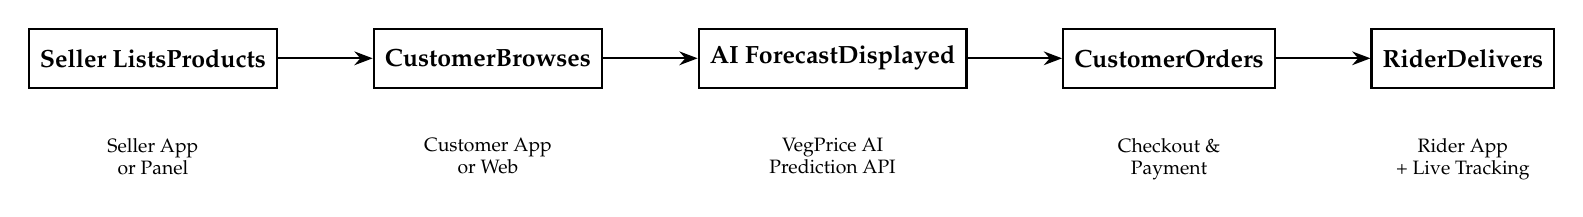
\begin{tikzpicture}[node distance=2.2cm and 0.5cm]
  \node[archnode, minimum width=2.0cm] (s1) {Seller Lists\\Products};
  \node[archnode, minimum width=2.0cm, right=1.2cm of s1] (s2) {Customer\\Browses};
  \node[archnode, minimum width=2.0cm, right=1.2cm of s2] (s3) {AI Forecast\\Displayed};
  \node[archnode, minimum width=2.0cm, right=1.2cm of s3] (s4) {Customer\\Orders};
  \node[archnode, minimum width=2.0cm, right=1.2cm of s4] (s5) {Rider\\Delivers};

  \draw[arrow] (s1)--(s2);
  \draw[arrow] (s2)--(s3);
  \draw[arrow] (s3)--(s4);
  \draw[arrow] (s4)--(s5);

  \node[below=0.5cm of s1,font=\scriptsize,align=center]
    {Seller App\\or Panel};
  \node[below=0.5cm of s2,font=\scriptsize,align=center]
    {Customer App\\or Web};
  \node[below=0.5cm of s3,font=\scriptsize,align=center]
    {VegPrice AI\\Prediction API};
  \node[below=0.5cm of s4,font=\scriptsize,align=center]
    {Checkout \&\\Payment};
  \node[below=0.5cm of s5,font=\scriptsize,align=center]
    {Rider App\\+ Live Tracking};
\end{tikzpicture}
\caption{Simplified end-to-end operational workflow}
\label{fig:workflow}
\end{figure}

\section{Step-by-Step Process Description}

\subsection{Phase 1: Seller Onboarding and Product Listing}

\begin{enumerate}
  \item A new seller registers on the platform. The Admin Panel receives a
        seller approval request and reviews the application.
  \item On approval, the seller subscribes to a plan (Free or paid tier).
  \item The seller uses the Seller App or Seller Panel to:
    \begin{itemize}
      \item Create one or more stores with addresses and operating hours.
      \item Define the delivery zones each store services.
      \item List vegetable products with price (Rs/kg), available variants
            (e.g., small bag, large bag), stock quantity, images, and
            product FAQs.
      \item Set tax rate overrides if permitted by admin.
    \end{itemize}
  \item All new products enter the admin approval queue. The Admin Panel
        reviews and approves or rejects each listing.
  \item Approved products become visible to customers in their geofenced zone.
\end{enumerate}

\subsection{Phase 2: Data Collection and Nightly Extraction}

\begin{enumerate}
  \item As customers place and receive orders, the eCommerce database records
        every transaction price for each vegetable per seller store.
  \item Each night at 01:00, the Integration Bridge cron job runs:
    \begin{itemize}
      \item Queries the eCommerce database for all delivered order item records
            since the previous extraction.
      \item Normalises records to the Supabase \texttt{price\_records} schema
            (date, vegetable\_name, market\_name, min/max/modal price,
            arrival\_qty).
      \item Upserts the records into Supabase \texttt{price\_records}.
    \end{itemize}
  \item The extraction run duration and record count are logged to Supabase
        \texttt{extraction\_log} for monitoring.
\end{enumerate}

\subsection{Phase 3: ML Model Retraining}

\begin{enumerate}
  \item At 02:00, the VegPrice AI scheduler triggers the daily retraining
        pipeline (\texttt{scripts/daily\_retrain.py}).
  \item For each of the 18 supported vegetables:
    \begin{itemize}
      \item Fetch all records from Supabase \texttt{price\_records}.
      \item Re-engineer features: lag, rolling, DOW, DOY, festival, weather.
      \item Retrain all five model classes (Linear Regression, Random Forest,
            XGBoost, LightGBM, Prophet).
      \item Evaluate each model on the last-30-day validation window
            by RMSE, MAE, MAPE, and direction accuracy.
      \item Recompute inverse-RMSE ensemble weights.
      \item Save updated \texttt{.pkl} artefacts to
            \texttt{data/model\_artifacts/\{vegetable\}/\{model\}.pkl}.
      \item Log metrics to Supabase \texttt{model\_metrics}.
    \end{itemize}
  \item Total retraining time: approximately 20--45 minutes for all 90 models.
\end{enumerate}

\subsection{Phase 4: AI Prediction Generation}

\begin{enumerate}
  \item After retraining, the scheduler triggers prediction generation for the
        next calendar day.
  \item For each vegetable, the ensemble model produces a weighted average
        prediction with confidence interval.
  \item The NVIDIA NIM API is called with a structured prompt containing:
        vegetable name, current price, 7-day price history, Chennai weather
        forecast, day-of-week, and festival proximity. The LLM returns a
        price prediction and reasoning trace.
  \item The AI prediction is saved to Supabase \texttt{predictions}:
    \begin{lstlisting}[language=Python, numbers=none]
supabase.table("predictions").insert({
    "vegetable_name":   veg,
    "prediction_date":  tomorrow.isoformat(),
    "predicted_price":  ai_price,
    "confidence_lower": lower,
    "confidence_upper": upper,
    "trend":            trend,         # up / down / stable
    "model_used":       nim_model_id,
    "reasoning":        lm_reasoning,
}).execute()
    \end{lstlisting}
  \item The Prediction Writer publishes the forecast to the eCommerce platform
        via \texttt{POST /api/product/price-forecast}.
\end{enumerate}

\subsection{Phase 5: Customer Experience with Price Forecast}

\begin{enumerate}
  \item The Customer App and Web fetch \texttt{GET /api/product/price-forecast}
        when rendering a vegetable product page.
  \item The forecast is displayed as:
    \begin{itemize}
      \item Current price (today's listed seller price).
      \item Tomorrow's predicted price with confidence range.
      \item Trend badge: green downward arrow (buy-now signal) or
            red upward arrow (wait signal).
      \item Optional: 7-day forecast chart fetched from
            \texttt{GET /weekly-forecast} on the VegPrice AI API.
    \end{itemize}
  \item Customers who have added a vegetable to their wishlist receive a
        push notification when the AI predicts a price drop exceeding a
        configured threshold.
\end{enumerate}

\subsection{Phase 6: Order Placement and Payment}

\begin{enumerate}
  \item The customer adds products to the cart (from one or multiple sellers
        within their active zone).
  \item At checkout:
    \begin{itemize}
      \item Zone eligibility is re-validated against the customer's saved
            delivery address.
      \item Applicable promo codes are validated.
      \item Tax and delivery charges are computed based on zone rules.
      \item Payment is processed via the configured gateway
            (card, UPI, wallet, or cash on delivery).
    \end{itemize}
  \item On payment confirmation, an order record is created in the eCommerce
        database with status \texttt{confirmed}.
  \item The seller receives a push notification via FCM.
\end{enumerate}

\subsection{Phase 7: Order Preparation and Rider Assignment}

\begin{enumerate}
  \item The seller updates the order status to \texttt{preparing} in the Seller
        App or Panel.
  \item When the order is ready (\texttt{ready\_for\_pickup}), the platform
        identifies available riders within the delivery zone.
  \item The nearest available rider receives a push notification; the rider
        accepts or rejects within 30 seconds.
  \item On acceptance, the order is assigned to that rider; status becomes
        \texttt{rider\_assigned}.
  \item If rejected, the next nearest available rider is notified (chain
        assignment). If no riders are available within the zone, the customer
        is notified with an estimated wait time.
\end{enumerate}

\subsection{Phase 8: Delivery and Tracking}

\begin{enumerate}
  \item The Rider App displays the seller's location and the customer's address
        on a turn-by-turn navigation map constrained to the geofenced zone.
  \item The rider's GPS coordinates are published to Supabase Realtime every
        5 seconds while the delivery is in progress.
  \item The Customer App displays the rider's live position on a map.
  \item Order status transitions: \texttt{rider\_assigned} →
        \texttt{picked\_up} → \texttt{out\_for\_delivery} → \texttt{delivered}.
  \item On delivery confirmation (rider marks as delivered), the customer
        receives a delivery notification and is prompted to submit a rating
        and review.
  \item The delivered transaction price is captured in the eCommerce database
        and will be included in the next nightly extraction cycle, feeding
        back into the prediction model.
\end{enumerate}

% =============================================================================
\chapter{Database Schema}
% =============================================================================

\section{Supabase (Prediction Engine Database)}

\begin{table}[H]
\centering
\caption{\texttt{price\_records} — Supabase}
\label{tab:price-records}
\begin{tabularx}{\textwidth}{@{} L{3.0cm} L{2.2cm} L{2.5cm} X @{}}
\toprule
\textbf{Column} & \textbf{Type} & \textbf{Constraint} & \textbf{Description} \\
\midrule
\texttt{id}              & INTEGER     & PK, AUTO      & Surrogate key \\
\texttt{date}            & VARCHAR(10) & NOT NULL, IDX & Date (YYYY-MM-DD) \\
\texttt{vegetable\_name} & VARCHAR(100)& NOT NULL, IDX & Vegetable slug \\
\texttt{market\_name}    & VARCHAR(200)& NULLABLE      & Seller store / market \\
\texttt{state}           & VARCHAR(100)& NULLABLE      & Tamil Nadu \\
\texttt{min\_price}      & FLOAT       & NULLABLE      & Minimum price (Rs/kg) \\
\texttt{max\_price}      & FLOAT       & NULLABLE      & Maximum price (Rs/kg) \\
\texttt{modal\_price}    & FLOAT       & NOT NULL      & Most common traded price \\
\texttt{arrival\_qty}    & FLOAT       & DEFAULT 0     & Quantity (tonnes / units) \\
\texttt{created\_at}     & DATETIME    & DEFAULT now() & Ingestion timestamp \\
\bottomrule
\end{tabularx}
\end{table}

\begin{table}[H]
\centering
\caption{\texttt{predictions} — Supabase (authoritative prediction store)}
\label{tab:predictions}
\begin{tabularx}{\textwidth}{@{} L{3.0cm} L{2.2cm} L{2.5cm} X @{}}
\toprule
\textbf{Column} & \textbf{Type} & \textbf{Constraint} & \textbf{Description} \\
\midrule
\texttt{id}               & INTEGER     & PK, AUTO      & Surrogate key \\
\texttt{vegetable\_name}  & VARCHAR(100)& NOT NULL, IDX & Vegetable slug \\
\texttt{prediction\_date} & VARCHAR(10) & NOT NULL      & Forecast target date \\
\texttt{predicted\_price} & FLOAT       & NOT NULL      & Predicted modal price \\
\texttt{confidence\_lower}& FLOAT       & NULLABLE      & 95\,\% CI lower bound \\
\texttt{confidence\_upper}& FLOAT       & NULLABLE      & 95\,\% CI upper bound \\
\texttt{trend}            & VARCHAR(10) & NULLABLE      & \texttt{up/down/stable} \\
\texttt{model\_used}      & VARCHAR(50) & NULLABLE      & Model identifier \\
\texttt{reasoning}        & TEXT        & NULLABLE      & LLM reasoning trace \\
\texttt{actual\_price}    & FLOAT       & NULLABLE      & Filled after date passes \\
\texttt{created\_at}      & DATETIME    & DEFAULT now() & Prediction creation time \\
\bottomrule
\end{tabularx}
\end{table}

\begin{table}[H]
\centering
\caption{\texttt{model\_metrics} — Supabase}
\label{tab:model-metrics}
\begin{tabularx}{\textwidth}{@{} L{3.0cm} L{2.2cm} L{2.5cm} X @{}}
\toprule
\textbf{Column} & \textbf{Type} & \textbf{Constraint} & \textbf{Description} \\
\midrule
\texttt{id}                  & INTEGER     & PK, AUTO & Row identifier \\
\texttt{model\_name}         & VARCHAR(50) & NOT NULL & e.g.\ \texttt{xgboost} \\
\texttt{vegetable\_name}     & VARCHAR(100)& NOT NULL & Target vegetable \\
\texttt{eval\_date}          & VARCHAR(10) & NOT NULL & Evaluation date \\
\texttt{rmse}                & FLOAT       & NULLABLE & Root mean squared error \\
\texttt{mae}                 & FLOAT       & NULLABLE & Mean absolute error \\
\texttt{mape}                & FLOAT       & NULLABLE & Mean abs. percentage error \\
\texttt{direction\_accuracy} & FLOAT       & NULLABLE & Trend accuracy (0--1) \\
\bottomrule
\end{tabularx}
\end{table}

\section{eCommerce Platform Database (Key Tables)}

\begin{table}[H]
\centering
\caption{eCommerce Platform Key Table Overview}
\label{tab:ec-schema}
\begin{tabularx}{\textwidth}{@{} L{3.4cm} X @{}}
\toprule
\textbf{Table} & \textbf{Key Columns and Purpose} \\
\midrule
\texttt{users}
  & id (UUID), name, email, phone, device\_token (FCM), role
    (customer/seller/rider/admin), created\_at. \\[4pt]
\texttt{sellers}
  & id, user\_id (FK), business\_name, subscription\_plan\_id,
    is\_approved, commission\_rate, wallet\_balance. \\[4pt]
\texttt{stores}
  & id, seller\_id (FK), name, address, lat, lng, operating\_hours (JSON),
    is\_active, delivery\_zone\_ids (array). \\[4pt]
\texttt{delivery\_zones}
  & id, name, polygon (GeoJSON), delivery\_fee, min\_order\_value,
    is\_active. \\[4pt]
\texttt{products}
  & id, store\_id (FK), name, category\_id, price, stock\_qty,
    is\_approved, is\_active, vegetable\_slug. \\[4pt]
\texttt{product\_variants}
  & id, product\_id (FK), attribute\_name, attribute\_value, price,
    stock\_qty. \\[4pt]
\texttt{orders}
  & id (UUID), customer\_id (FK), status, total\_amount,
    delivery\_address (JSON), payment\_method, delivered\_at. \\[4pt]
\texttt{order\_items}
  & id, order\_id (FK), product\_id (FK), variant\_id, quantity, price,
    store\_id. \\[4pt]
\texttt{price\_forecasts}
  & id, vegetable\_slug, prediction\_date, predicted\_price,
    confidence\_lower, confidence\_upper, trend, model\_used,
    published\_at. \textit{Written by the prediction engine.} \\[4pt]
\texttt{riders}
  & id, user\_id (FK), zone\_id, is\_available, current\_lat,
    current\_lng, wallet\_balance. \\[4pt]
\texttt{delivery\_assignments}
  & id, order\_id (FK), rider\_id (FK), assigned\_at, picked\_up\_at,
    delivered\_at, status. \\[4pt]
\texttt{ratings}
  & id, order\_id (FK), product\_rating (1--5), delivery\_rating (1--5),
    review\_text. \\[4pt]
\texttt{subscription\_plans}
  & id, name, price, billing\_cycle, max\_products, max\_stores,
    features (JSON). \\[4pt]
\texttt{notifications}
  & id, user\_id (FK), title, body, type, is\_read, sent\_at. \\
\bottomrule
\end{tabularx}
\end{table}

% =============================================================================
\chapter{API Documentation}
% =============================================================================

\section{VegPrice AI Prediction API}

\textbf{Production base URL:}
\texttt{https://chennai-vegetable-price-prediction.vercel.app}

\begin{longtable}{@{} C{1.4cm} L{6.0cm} L{6.8cm} @{}}
\caption{VegPrice AI Complete Endpoint Reference}
\label{tab:pred-endpoints-full} \\
\toprule
\textbf{Method} & \textbf{Endpoint} & \textbf{Description} \\
\midrule
\endfirsthead
\toprule
\textbf{Method} & \textbf{Endpoint} & \textbf{Description} \\
\midrule
\endhead
\bottomrule
\endlastfoot
GET    & \texttt{/}                                   & API name and version. \\[3pt]
GET    & \texttt{/health}                             & Status and Supabase connectivity. \\[3pt]
GET    & \texttt{/weather}                            & Real-time Chennai weather (Open-Meteo). \\[3pt]
GET    & \texttt{/vegetables}                         & List of 18 supported vegetable slugs. \\[3pt]
GET    & \texttt{/predict?vegetable=X\&market=Y}      & Supabase-first prediction; ML fallback. \\[3pt]
GET    & \texttt{/ai-predict?vegetable=X}             & NVIDIA NIM LLM prediction + reasoning. \\[3pt]
GET    & \texttt{/get-current-price?vegetable=X}      & Latest price from \texttt{price\_records}. \\[3pt]
GET    & \texttt{/get-current-price/market-comparison}& All markets sorted by current price. \\[3pt]
GET    & \texttt{/price-history?vegetable=X\&days=30} & Last $N$ days of price records. \\[3pt]
GET    & \texttt{/weekly-forecast?vegetable=X}        & 7-day forecast array. \\[3pt]
GET    & \texttt{/dashboard}                          & All 18 vegetables; top rising/falling. \\[3pt]
POST   & \texttt{/scan-image}                         & Image → NVIDIA vision → veg + price. \\[3pt]
GET    & \texttt{/test-ai}                            & NVIDIA NIM connectivity test. \\[3pt]
POST   & \texttt{/alerts}                             & Create FCM price alert subscription. \\[3pt]
GET    & \texttt{/alerts/\{user\_id\}}                & List user's active alerts. \\[3pt]
DELETE & \texttt{/alerts/\{alert\_id\}}               & Remove a price alert. \\
\end{longtable}

\section{eCommerce Platform API (Integration-Relevant)}

\begin{table}[H]
\centering
\caption{eCommerce API Endpoints Used by the Integration Bridge}
\label{tab:ec-api}
\begin{tabularx}{\textwidth}{@{} C{1.4cm} L{6.0cm} X @{}}
\toprule
\textbf{Method} & \textbf{Endpoint} & \textbf{Description} \\
\midrule
GET  & \texttt{/api/price-records?since=DATE}
     & Returns delivered order price records since the given date,
       normalised for ingestion into Supabase. \\[3pt]
POST & \texttt{/api/product/price-forecast}
     & Accepts a prediction payload and stores it in the
       \texttt{price\_forecasts} table. \\[3pt]
GET  & \texttt{/api/product/price-forecast?vegetable=X}
     & Returns the current stored forecast for a vegetable. \\[3pt]
GET  & \texttt{/api/zones/active}
     & Returns all active delivery zones with polygon boundaries. \\[3pt]
GET  & \texttt{/api/seller/products?category=vegetable}
     & Returns all active vegetable product listings across all sellers. \\[3pt]
POST & \texttt{/api/notifications/send}
     & Sends a push notification to a user segment (used by alert system). \\
\bottomrule
\end{tabularx}
\end{table}

\section{API Response Examples}

\subsection{Price Forecast Response (Prediction API)}

\begin{lstlisting}[language=Python, numbers=none,
  caption={GET /predict response schema}]
{
  "vegetable":        "tomato",
  "prediction_date":  "2026-04-12",
  "current_price":    42.0,
  "predicted_price":  44.50,
  "confidence_lower": 40.00,
  "confidence_upper": 49.00,
  "trend":            "up",
  "trend_badge":      "up",
  "model_name":       "meta/llama-3.1-8b-instruct",
  "reasoning":        "Tomato prices are expected to rise on Tuesday due to
                       reduced arrivals following weekend heavy rainfall in
                       Krishnagiri district. Festival demand from Pongal
                       preparations adds 8-12% upward pressure."
}
\end{lstlisting}

\subsection{Dashboard Response (Prediction API)}

\begin{lstlisting}[language=Python, numbers=none,
  caption={GET /dashboard response schema}]
{
  "total_vegetables": 18,
  "rising_count":     7,
  "falling_count":    6,
  "stable_count":     5,
  "top_rising":  [
    {"vegetable": "tomato",  "current_price": 42.0, "change_pct":  5.2},
    {"vegetable": "ginger",  "current_price": 120.0,"change_pct":  3.8}
  ],
  "top_falling": [
    {"vegetable": "onion",   "current_price": 35.0, "change_pct": -3.1},
    {"vegetable": "cabbage", "current_price": 18.0, "change_pct": -2.6}
  ],
  "all_predictions": [ /* 18 PredictionResponse objects */ ]
}
\end{lstlisting}

% =============================================================================
\chapter{Deployment and DevOps}
% =============================================================================

\section{System Deployment Overview}

\begin{table}[H]
\centering
\caption{Deployment Environment Summary}
\label{tab:deployment}
\begin{tabularx}{\textwidth}{@{} L{3.4cm} L{3.2cm} X @{}}
\toprule
\textbf{Component} & \textbf{Hosting} & \textbf{Details} \\
\midrule
VegPrice AI API        & Vercel Serverless & Auto-deploy on push to \texttt{main}; Python stdlib only \\
eCommerce Backend API  & Cloud Server / VPS & Node.js or Laravel; PM2 process manager \\
Supabase Database      & Supabase Cloud    & Managed PostgreSQL; REST + Realtime + Auth \\
eCommerce Database     & Managed PostgreSQL& Separate from Supabase; app-specific schema \\
Customer App (Android) & EAS Build + APK   & Preview APK for sideload; AAB for Play Store \\
Customer App (iOS)     & EAS Build + IPA   & TestFlight for beta; App Store for production \\
Seller App             & EAS Build         & Same as Customer App build pipeline \\
Rider App              & EAS Build         & Separate EAS project or profile \\
Admin/Seller Web Panel & Vercel / Netlify  & Static export of React application \\
ML Worker              & Docker (ml-worker)& APScheduler nightly retraining; shares data volume \\
Redis Cache            & Docker / Redis Cloud & 256 MB LRU; prediction response caching \\
\bottomrule
\end{tabularx}
\end{table}

\section{VegPrice AI Vercel Deployment}

\begin{itemize}
  \item \texttt{vercel.json}: single rewrite routing all requests to
        \texttt{api/index.py}.
  \item \texttt{api/index.py}: Python stdlib only; zero cold-start overhead
        from package installation.
  \item Auto-deployed on every push to the \texttt{main} GitHub branch.
  \item Environment variables set in Vercel dashboard:
        \texttt{NVIDIA\_API\_KEY}, \texttt{SUPABASE\_URL},
        \texttt{SUPABASE\_SERVICE\_ROLE\_KEY},
        \texttt{ECOMMERCE\_API\_BASE}, \texttt{ECOMMERCE\_API\_KEY}.
\end{itemize}

\section{Docker Compose (Local Full Stack)}

\begin{table}[H]
\centering
\caption{Docker Compose Services}
\label{tab:docker}
\begin{tabularx}{\textwidth}{@{} L{2.6cm} L{3.0cm} X @{}}
\toprule
\textbf{Service} & \textbf{Image} & \textbf{Description} \\
\midrule
\texttt{api}       & Dockerfile.api    & FastAPI on port 8000; mounts data and config. \\
\texttt{redis}     & redis:7-alpine    & 256 MB LRU cache; 15-minute prediction TTL. \\
\texttt{ml-worker} & Dockerfile.ml     & APScheduler; nightly retraining at 02:00. \\
\texttt{ecommerce} & app/Dockerfile    & eCommerce backend API on port 3000. \\
\texttt{ec-db}     & postgres:15       & eCommerce PostgreSQL database. \\
\texttt{bridge}    & Dockerfile.bridge & Integration Bridge cron container. \\
\bottomrule
\end{tabularx}
\end{table}

\section{EAS Build Profiles}

\begin{table}[H]
\centering
\caption{EAS Build Profiles for Mobile Apps}
\label{tab:eas}
\begin{tabularx}{\textwidth}{@{} L{2.4cm} L{2.2cm} L{1.8cm} X @{}}
\toprule
\textbf{Profile} & \textbf{Platform} & \textbf{Output} & \textbf{Use Case} \\
\midrule
\texttt{preview}    & Android & APK & Internal testing and sideloading \\
\texttt{production} & Android & AAB & Google Play Store submission \\
\texttt{development}& Both    & APK/IPA & Dev client with fast refresh \\
\texttt{ios-preview}& iOS     & IPA & TestFlight beta distribution \\
\bottomrule
\end{tabularx}
\end{table}

\section{Nightly Cron Schedule}

\begin{table}[H]
\centering
\caption{Scheduled Job Timeline}
\label{tab:cron}
\begin{tabularx}{\textwidth}{@{} L{2.4cm} L{3.0cm} X @{}}
\toprule
\textbf{Time (IST)} & \textbf{Job} & \textbf{Description} \\
\midrule
00:30 & Zone price sync     & Fetch latest seller prices from eCommerce API. \\
01:00 & Data extraction     & Extract delivered order price records to Supabase. \\
02:00 & ML retraining       & Retrain all 90 model artefacts. \\
04:00 & Prediction publish  & Generate next-day forecasts; publish to eCommerce. \\
06:00 & Alert evaluation    & Compare current prices to \texttt{price\_alerts}; send FCM. \\
\bottomrule
\end{tabularx}
\end{table}

% =============================================================================
\chapter{Security}
% =============================================================================

\section{Authentication Model}

\begin{table}[H]
\centering
\caption{Authentication Mechanisms by Component}
\label{tab:auth}
\begin{tabularx}{\textwidth}{@{} L{3.4cm} X @{}}
\toprule
\textbf{Component} & \textbf{Authentication Mechanism} \\
\midrule
Customer App / Web
  & Supabase Auth (email/password, Google OAuth, phone OTP). JWT stored
    in AsyncStorage; refreshed automatically. \\[4pt]
Seller App / Panel
  & Same Supabase Auth; role claim \texttt{seller} validated on the backend.
    Admin approves seller role manually. \\[4pt]
Rider App
  & Supabase Auth with role claim \texttt{rider}; zone assignment validated
    on login. \\[4pt]
Admin Panel
  & Supabase Auth with role claim \texttt{admin}; additional per-module
    permission flags in \texttt{admin\_permissions} table. \\[4pt]
Integration Bridge
  & API key authentication (\texttt{X-Bridge-Key} header) on the eCommerce
    integration endpoints. Key rotated monthly. \\[4pt]
VegPrice AI API
  & \texttt{NVIDIA\_API\_KEY} for LLM calls; \texttt{SUPABASE\_SERVICE\_ROLE\_KEY}
    for database writes. User-facing endpoints are public. \\[4pt]
NVIDIA NIM
  & Bearer token (\texttt{Authorization: Bearer nvapi-\ldots}) in every
    AI request. \\
\bottomrule
\end{tabularx}
\end{table}

\section{Security Controls}

\begin{itemize}
  \item \textbf{CORS}: eCommerce API restricts origins to known app domains.
        VegPrice AI API currently allows all origins (planned: restrict to
        eCommerce domain).
  \item \textbf{Rate limiting}: \texttt{slowapi} per-IP limiting on the
        FastAPI deployment. Vercel platform-level DDoS protection on the
        serverless handler.
  \item \textbf{Input validation}: All vegetable slugs sanitised
        (\texttt{.lower().replace(" ", "\_")}); image payloads capped at
        10\,MB; zone polygons validated for closure and minimum vertex count.
  \item \textbf{Secrets management}: All keys in \texttt{.env} (gitignored)
        locally; Vercel environment variables and server environment variables
        in production. Never committed to source control.
  \item \textbf{Row-level security}: Supabase RLS policies enforce that users
        can only read/write their own \texttt{price\_alerts} and
        \texttt{notifications} rows.
  \item \textbf{Payment security}: All payment processing is delegated to
        PCI-compliant payment gateway SDKs; no card data touches the
        application servers.
\end{itemize}

% =============================================================================
\chapter{Testing Strategy}
% =============================================================================

\section{Test Coverage}

\begin{table}[H]
\centering
\caption{Test Suite Coverage}
\label{tab:tests}
\begin{tabularx}{\textwidth}{@{} L{5.0cm} L{3.8cm} L{4.8cm} @{}}
\toprule
\textbf{Test File / Suite} & \textbf{Coverage Area} & \textbf{Framework} \\
\midrule
\texttt{tests/test\_api.py}               & VegPrice AI routes      & pytest + httpx \\
\texttt{tests/test\_models.py}            & ML model load/predict   & pytest \\
\texttt{tests/test\_data\_pipeline.py}    & Data extraction/features & pytest \\
\texttt{tests/test\_integration\_bridge.py}& eCommerce→Supabase sync & pytest + mock \\
\texttt{tests/test\_prediction\_publish.py}& Supabase→eCommerce push & pytest + mock \\
\texttt{tests/test\_vision.py}            & NVIDIA vision scan      & pytest \\
\texttt{ecommerce/tests/order.spec.js}    & Order placement E2E     & Jest + Supertest \\
\texttt{ecommerce/tests/zone.spec.js}     & Zone eligibility logic  & Jest \\
\texttt{ecommerce/tests/commission.spec.js}& Commission calculation  & Jest \\
\bottomrule
\end{tabularx}
\end{table}

\section{Running Tests}

\begin{lstlisting}[language=bash, numbers=none,
  caption={Test execution commands}]
# VegPrice AI unit and integration tests
source venv/bin/activate
pytest tests/ -v --cov=api --cov=src --cov-report=html

# Integration bridge tests (mock eCommerce DB)
pytest tests/test_integration_bridge.py -v

# eCommerce backend tests
cd ecommerce && npm test
\end{lstlisting}

\section{Code Quality}

\begin{itemize}
  \item \textbf{ruff} --- Python lint; rules E/F/I/UP; line length 100.
  \item \textbf{black} --- Python formatter; target Python 3.11.
  \item \textbf{mypy} --- Static type checking.
  \item \textbf{TypeScript strict mode} --- All mobile source files
        type-checked via \texttt{tsc --noEmit}.
  \item \textbf{ESLint} --- JavaScript/TypeScript lint for the eCommerce
        backend and web panels.
\end{itemize}

% =============================================================================
\chapter{Known Issues and Roadmap}
% =============================================================================

\section{Current Limitations}

\begin{table}[H]
\centering
\caption{Known Limitations}
\label{tab:limitations}
\begin{tabularx}{\textwidth}{@{} L{4.2cm} X @{}}
\toprule
\textbf{Limitation} & \textbf{Description and Planned Resolution} \\
\midrule
Nightly-only extraction
  & Price data flows from eCommerce to Supabase only once per night.
    Real-time streaming via eCommerce webhooks is planned. \\[4pt]
No user authentication (AI API)
  & The VegPrice AI API endpoints are public. Planned: API key auth for
    the eCommerce bridge; Supabase Auth for end-users. \\[4pt]
Days 2--7 forecast (ML only)
  & Only day-1 forecast uses NVIDIA NIM; days 2--7 use the seasonal
    ML ensemble. Multi-day LLM trajectory prompt is planned. \\[4pt]
Alert scheduling
  & FCM alert records are stored but no server cron yet evaluates current
    prices against thresholds. Planned: 30-minute evaluation cron. \\[4pt]
EAS free-tier queue
  & Android cloud builds can wait 30--60 minutes. Planned: EAS paid tier
    or local Gradle build environment. \\[4pt]
No iOS build yet
  & Rider and Seller apps target Android only at launch. iOS requires an
    Apple Developer account. \\[4pt]
CORS open policy
  & VegPrice AI allows all origins. Planned: restrict to eCommerce
    domain once auth is integrated. \\
\bottomrule
\end{tabularx}
\end{table}

\section{Technical Debt}

\begin{itemize}
  \item \texttt{api/index.py} (Vercel) and \texttt{api/main.py} (FastAPI)
        have diverged; \texttt{/price-history} and \texttt{/test-ai} are
        missing from FastAPI. Resolution: add missing endpoints.
  \item Integration Bridge uses a hard-coded extraction window; should use
        a \texttt{last\_extracted\_at} checkpoint table.
  \item No unique constraint on \texttt{(vegetable\_name, prediction\_date)}
        in Supabase \texttt{predictions}; duplicate rows possible.
\end{itemize}

\section{Planned Features}

\begin{enumerate}
  \item \textbf{Real-time price streaming} --- eCommerce platform emits a
        webhook on each order settlement; Integration Bridge writes the price
        record immediately to Supabase; prediction updates in near real-time.
  \item \textbf{Multi-day AI forecast} --- Ask NVIDIA NIM for a 7-day price
        trajectory in a single chain-of-thought prompt.
  \item \textbf{Demand forecasting} --- Predict order volume per zone per
        vegetable to help sellers plan inventory.
  \item \textbf{Dynamic pricing suggestion} --- Suggest optimal seller listing
        prices based on predicted next-day prices and competitor analysis.
  \item \textbf{iOS release} --- Expo managed workflow with minimal code changes.
  \item \textbf{Scheduled alert evaluation} --- Server-side cron comparing
        current prices to \texttt{price\_alerts} and dispatching FCM pushes.
  \item \textbf{Supabase Auth integration} --- Full user authentication for the
        VegPrice AI API; per-user predictions and private alert management.
  \item \textbf{Google Play and App Store publishing} --- Production builds via
        EAS Submit and Fastlane metadata management.
  \item \textbf{Vendor price input} --- Allow sellers to submit actual market
        prices directly via the Seller App; instant Supabase record ingestion.
  \item \textbf{Seasonal calendar view} --- Heat-map calendar showing
        historically cheapest months per vegetable.
\end{enumerate}

% =============================================================================
\appendix
% =============================================================================

\chapter{Supported Vegetables}
\label{app:vegetables}

\begin{table}[H]
\centering
\caption{All 18 Supported Vegetable Slugs}
\label{tab:vegs}
\begin{tabularx}{\textwidth}{@{} C{0.8cm} L{3.6cm} C{0.8cm} L{3.6cm} C{0.8cm} L{3.6cm} @{}}
\toprule
\textbf{\#} & \textbf{Slug} & \textbf{\#} & \textbf{Slug} & \textbf{\#} & \textbf{Slug} \\
\midrule
1  & \texttt{tomato}        &  7 & \texttt{brinjal}      & 13 & \texttt{ladies\_finger} \\
2  & \texttt{onion}         &  8 & \texttt{cabbage}      & 14 & \texttt{bitter\_gourd}  \\
3  & \texttt{potato}        &  9 & \texttt{carrot}       & 15 & \texttt{bottle\_gourd}  \\
4  & \texttt{garlic}        & 10 & \texttt{cauliflower}  & 16 & \texttt{raw\_banana}    \\
5  & \texttt{ginger}        & 11 & \texttt{beans}        & 17 & \texttt{drumstick}      \\
6  & \texttt{green\_chilli} & 12 & \texttt{coriander}    & 18 & \texttt{tapioca}        \\
\bottomrule
\end{tabularx}
\end{table}

\chapter{Environment Variables}
\label{app:envvars}

\begin{longtable}{@{} L{5.5cm} C{2.0cm} L{6.7cm} @{}}
\caption{Complete Environment Variable Reference}
\label{tab:env-full} \\
\toprule
\textbf{Variable} & \textbf{Required} & \textbf{Description} \\
\midrule
\endfirsthead
\toprule
\textbf{Variable} & \textbf{Required} & \textbf{Description} \\
\midrule
\endhead
\bottomrule
\endlastfoot
\texttt{SUPABASE\_URL}                 & Yes          & Supabase project REST URL \\
\texttt{SUPABASE\_ANON\_KEY}           & Yes          & Public anon key \\
\texttt{SUPABASE\_SERVICE\_ROLE\_KEY}  & Yes          & Admin write key --- server only \\
\texttt{DATABASE\_URL}                 & FastAPI      & asyncpg connection string \\
\texttt{NVIDIA\_API\_KEY}              & Yes (AI)     & Free at \texttt{build.nvidia.com} \\
\texttt{REDIS\_URL}                    & FastAPI      & Default: \texttt{redis://localhost:6379/0} \\
\texttt{SECRET\_KEY}                   & FastAPI      & JWT signing secret (32+ chars) \\
\texttt{FCM\_SERVER\_KEY}              & Alerts       & Firebase Cloud Messaging key \\
\texttt{ECOMMERCE\_API\_BASE}          & Bridge       & eCommerce backend base URL \\
\texttt{ECOMMERCE\_API\_KEY}           & Bridge       & API key for integration endpoints \\
\texttt{ECOMMERCE\_DB\_URL}            & Bridge       & Direct DB connection for extraction \\
\texttt{ENVIRONMENT}                   & No           & \texttt{development} or \texttt{production} \\
\texttt{LOG\_LEVEL}                    & No           & \texttt{INFO} / \texttt{DEBUG} \\
\texttt{MODEL\_ARTIFACTS\_PATH}        & No           & Default: \texttt{data/model\_artifacts} \\
\texttt{DATA\_FEATURES\_PATH}          & No           & Default: \texttt{data/features} \\
\end{longtable}

\chapter{Glossary}
\label{app:glossary}

\begin{description}
  \item[Agmarknet]
    Indian Government portal providing historical mandi arrival and price data.
  \item[APK / AAB]
    Android Package (sideload) and Android App Bundle (Play Store).
  \item[AsyncStorage]
    React Native key-value storage backed by SQLite on Android.
  \item[DOW / DOY]
    Day of Week (0--6) / Day of Year (1--365); used as ML seasonality features.
  \item[EAS]
    Expo Application Services; cloud build and OTA update platform.
  \item[Ensemble]
    Combination of predictions from five ML models via inverse-RMSE weights.
  \item[FCM]
    Firebase Cloud Messaging; Google's cross-platform push notification service.
  \item[Geofencing]
    GPS polygon boundary defining a delivery zone; orders and rider navigation
    are constrained within the boundary.
  \item[HyperLocal]
    Commerce model where buyers and sellers are within a defined geographic
    zone; delivery times are short (minutes to hours).
  \item[Koyambedu]
    Chennai's primary wholesale vegetable market; one of Asia's largest.
  \item[MAPE]
    Mean Absolute Percentage Error; primary ML model selection metric.
  \item[Modal Price]
    Most frequently traded price in a market session; the ML target variable.
  \item[M3]
    Material Design 3; Google design system used in the mobile apps.
  \item[NVIDIA NIM]
    NVIDIA Inference Microservices; hosted LLM and vision model API.
  \item[RLS]
    Row Level Security; Supabase/PostgreSQL per-row access control.
  \item[Supabase]
    Open-source Firebase alternative on PostgreSQL; provides REST, Realtime,
    Auth, and Storage.
  \item[Vercel Serverless]
    Edge-deployed Python functions with zero cold-start dependency overhead.
  \item[Webhook]
    HTTP callback sent by the eCommerce platform to the Integration Bridge
    immediately after a price-relevant event (order settlement).
\end{description}

\end{document}
